% \Image{Capa do livro (; )}{PNLD2022-015-01.png}

% \Image{Ilustração do livro (Kalinka/Vera Ermoláieva; Kalinka)}{PNLD2022-015-04.png}
% \Image{Ilustração do livro (Kalinka/Vera Ermoláieva; Kalinka)}{PNLD2022-015-05.png}
% \Image{Ilustração do livro (Kalinka/Vera Ermoláieva; Kalinka)}{PNLD2022-015-06.png}



\documentclass[11pt]{extarticle}
\usepackage{manualdoprofessor}
\usepackage{fichatecnica}
\usepackage{lipsum,media9}
\usepackage[justification=raggedright]{caption}
\usepackage[one]{bncc}
\usepackage[kalinka]{../edlab}
\usepackage{marginnote}
\usepackage{pdfpages}
\usepackage[printwatermark]{xwatermark}
\newwatermark[pagex=2]{
\includegraphics[scale=3.3]{watermarks/test-a.png}}	% página específica
%\newwatermark[oddpages]{
\includegraphics{watermarks/test-a.png}}			% páginas ímpars
%\newwatermark[evenpages]{
\includegraphics{watermarks/test-a.png}}			% págimas pares
\newwatermark[allpages]{
\includegraphics[scale=3.3]{watermarks/test-b.png}}

\pagecolor{cyan!0!magenta!10!yellow!28!black!28!}

\newcommand{\AutorLivro}{Vera Ermoláieva}
\newcommand{\TituloLivro}{Cachorrinhos}
\newcommand{\Tema}{Animais da fauna local, nacional e mundial}
\newcommand{\Genero}{Narrativos: fábulas originais; da literatura universal e da tradição popular; etc}
%\newcommand{\imagemCapa}{./images/PNLD0001-01.png}
\newcommand{\issnppub}{978-65-86862-10-2}
\newcommand{\issnepub}{978-65-86862-13-3}
% \newcommand{\fichacatalografica}{PNLD0001-00.png}
\newcommand{\colaborador}{{Paulo Pompermaier e Renier Silva}}

\begin{document}

\title{\TituloLivro}
\author{\AutorLivro}
\def\authornotes{\colaborador}

\date{}
\maketitle

%\begin{abstract}\addcontentsline{toc}{section}{Carta ao professor}
%\pagebreak

\tableofcontents



\section{Sobre o livro}

%550 caracteres
\paragraph{O livro} \textit{Cachorrinhos} (1929), de Vera Ermoláieva, figura-chave da vanguarda russa, faz parte de uma série de livros ilustrados russos do início do século 20 que anunciou o design moderno.
A simplicidade da composição e a complexidade conceitual definem a obra. Mas isso não
significa que ela não vai interessar aos pequenos! Afinal, é um livro que possibilita
estimular o interesse da criança em ouvir histórias e mostrar as relações entre
escrita e imagem; expor a criança a diferentes manifestações artísticas (pintura, desenho, design, de modo que ela comece a desenvolver senso estético; potencializar conhecimentos matemáticos (contagem, ordenação, relações entre quantidades, dimensões, medidas, reconhecimento de formas geométricas, reconhecimento de numerais); aguçar a curiosidade pelo livro; promover o contato com a cultura russa.


%822 caracteres
\paragraph{Descrição} O livro começa com uma conversa sobre o nome dos cachorros. Existe um nome apropriado para os cachorros? pergunta-se o narrador. Pode um cachorrinho que vive dentro de casa se chamar Coronel, e um cachorrão de guarda se chamar Zizi? As perguntas são todas abertas e ficam sugeridas para os leitores pensarem a respeito. Depois, o livro passa a narrar a história de um menino, o mesmo que se perguntava sobre o nome dos animais.
O jovem vai para uma exposição de cachorros. Admirado, ele tenta colocar todos os cães no
seu caderno. São tantos que se vê obrigado a desenhá-los cada vez menores. À medida que os
números aumentam, os cachorrinhos diminuem. Cada um tem uma expressão, um
movimento, um nome e olha para um lado. Ao mesmo tempo, o conjunto deles forma
composições livres no espaço branco da página.

%411 caracteres
\paragraph{Competências}
O livro \textit{Cachorrinhos} desenvolve e explora diferentes competências relacionadas às formas, tamanhos e perspectivas. Com a disposição das figuras caninas nas páginas, a criança tem contato e percebe os diferentes tamanhos das figuras, traçando comparações e divergências entre as figuras. Os tamanhos variados também relacionam-se à perspectiva, pois criam jogos visuais em que as figuras parecem maiores e mais próximas e menores e mais distantes. Com a contagem progressiva dos cachorros, sempre com o múltiplo do número precedente (2, 4, 8, 16, 32 etc.), mobiliza-se a apreensão de quantidade e princípios de agrupamento,''


%862 caracteres
\paragraph{Aprofundamento} Este material tem a 
intenção de contribuir para que você consiga desenvolver um trabalho aprofundado 
com esta obra na sala de aula. Você encontrará informações sobre a autora, sobre 
o gênero e sobre os temas trabalhados ao longo do livro. Apresentaremos também 
algumas propostas de trabalho para a sala de aula que você poderá explorar livremente, 
da forma que considerar mais apropriada para os seus estudantes. Para a prática 
da Literacia Familiar, oferecemos um guia que pode ajudar nas orientações aos 
responsáveis pela criança, para incentivar o gosto pela leitura e contribuir para 
que os estudantes desenvolvam em casa habilidades que serão importantes no momento 
da alfabetização. Por fim, você encontrará sugestões de livros, artigos e sites 
selecionados para enriquecer a sua experiência de leitura e, 
consequentemente, a de seus estudantes.



\section{Sobre os autores}

\Image{Foto da autora e ilustradora (Kalinka; Kalinka)}{PNLD2022-015-02.png}

%532 caracteres
\paragraph{A autora} A pintora, ilustradora e pedagoga Vera Ermoláieva nasceu em 1893 na província de Sarátov, no sul da Rússia. Quando pequena, sofreu uma queda de um cavalo que a deixou com as pernas paralisadas. Os pais a levaram à Europa em busca de uma cura, mas, sem sucesso, voltaram para a Rússia em 1904, onde ela concluiu o ginásio. A dificuldade de locomoção nunca limitou a vida de Vera Ermoláieva, que, ativa e generosa, enveredou por várias áreas da pintura e das artes gráficas.
Em 1914, passou uma temporada em Paris, interessada pela linguagem de artistas
como Cézanne, Picasso e Braque. Ermoláieva estudou pintura em São Petersburgo no estúdio de M. Bernstein, na época popular entre artistas interessados por futurismo e por outras tendências modernas; formou-se antropóloga em 1917. Organizou, ao lado de outros pintores representativos, o coletivo “Hoje” (1918), que produziu livros infantis com base na cultura popular russa (\textit{lubók}) por meio
de processos gráficos artesanais. São livros que se tornaram referência para artistas e
pesquisadores russos, apresentando uma interação mais orgânica entre texto e imagem. No
ano seguinte foi trabalhar no Escola de Pintura do Povo de Vítebsk (atual Bielorrússia), onde
lecionaram Chagall e Malévitch, de quem ela foi discípula e colaboradora. Ermoláieva fez parte
do grupo \textsc{unovis} (Consolidadores da nova arte), um laboratório suprematista. De volta a São
Petersburgo, lecionou no Instituto Estatal de Educação Artística (\textsc{guinkhuk}), ao lado de
grandes mestres, е trabalhou como ilustradora.
Figura ativa da vanguarda russa, Vera Ermoláieva trabalhou nas melhores revistas
infantojuvenis soviéticas e ilustrou livros de muitos autores. Neles usou linguagens pictóricas diferentes --- fauvismo, cubismo, construtivismo ---, tornando-se referência da escola gráfica de Leningrado e ajudando a desenvolver o novo tipo de livro ilustrado para crianças que surgiu na
Rússia na década de 1920. Produzidas por grandes artistas, são obras hoje apreciadas por
colecionadores e designers do mundo todo.
Em 1934, em meio à censura stalinista, Ermoláieva foi acusada de propagar ideias
antissoviéticas em arte e acabou presa, com membros do grupo “realismo pictórico-escultural”, seguidores de Malévitch. Morreu fuzilada em 1937 em um campo de prisioneiros.
Em 2013, foi criada em Moscou a Fundação Vera Ermoláieva, para iniciativas de artistas
contemporâneas.

%313 caracteres
\paragraph{A designer} Karina Aoki, nascida em São Paulo em 1977, é formada em Arquitetura e Urbanismo pela \textsc{fau-usp}. Atuou como diretora de arte e coordenadora de estúdio da São Paulo Criação -- Rafic Farah durante oito anos, atendendo clientes como Mitsubishi Motors do Brasil, Fundação Roberto Marinho, Fast Shop, Casa do Saber, Escola da Cidade, Museu de Arte Brasileira da \textsc{faap}, restaurantes Arabia, Spot e Ritz, marcas de moda Maria Bonita, Mandi, Lucy in the Sky e
Brooksfield Donna, cinema \textsc{hsbc}/Belas Artes, e o designer Carlos Motta. Foi também editora de arte da revista Casa Vogue (Edições Globo Condé Nast) por seis anos e supervisora de arte do departamento de literatura da editora \textsc{ftd} Educação, sendo responsável por cerca de 70 títulos. Atualmente desenvolve projetos independentes nas áreas de identidade visual, embalagem, expografia e editorial.

Karina Aoki adaptou a capa de modo que a criança brasileira tivesse acesso ao
desenho original. O miolo ganhou dinamismo com a história sendo contada por frases curtas
intercaladas por ilustrações e símbolos de pontuação, incentivando a criança a estabelecer
relações entre imagem e conceito.

%358 caracteres
\paragraph{O tradutor} 
Moissei Mountian, nascido em 1948 na \textsc{urss} (Moldávia), é formado em engenharia civil. Em 1972, mudou-se com sua esposa, Sofia Mountian, para o Brasil, onde em 2008 fundou com sua filha Daniela a editora Kalinka, dedicada à literatura russa, e começou a trabalhar como tradutor. É parte do conselho editorial da Kalinka, tendo trazido nomes como Fiódor Sologub, Leonid Dobýtchin e Friedrich Gorenstein aos leitores brasileiros. Foi indicado duas vezes ao Prêmio Jabuti pelas traduções de \textit{O Diabo Mesquinho}, de Fiódor Sologub (Kalinka, 2008), e \textit{Os sonhos teus vão acabar contigo: prosa, poesia,teatro}, de Daniil Kharms (Kalinka, 2103, com Aurora Fornoni Bernardini e Daniela Mountian). Também traduziu \textit{Encontros com Liz e outras histórias}, de Leonid Dobýtchin (Kalinka, 2009), \textit{Diário de um escritor (1873): Meia carta de um
sujeito}, de Fiódor Dostoiévski (Hedra, 2016), e \textit{A ressurreição do lariço: Contos de Kolimá 5}, de Varlam Chalámov (Ed. 34, 2016), os dois últimos em parceria com Daniela. Com Irineu Franco Perpetuo verteu Salmo, de \textit{Friedrich Gorenstein} (indicado ao prêmio de tradução “Lendo a Rússia”, do Instituto de Tradução de Moscou).
 
Em sua versão, o tradutor Moissei Mountian buscou aproximar o texto russo da criança
brasileira, mantendo o humor, a leveza e a ludicidade do original.

\section{Sobre o gênero}

%55 caracteres
\paragraph{O gênero} O gênero deste livro é \textit{narrativa}. 

\Image{O gênero da narrativa proporciona ao leitor uma abertura ao mundo. (Pixabay/Tumisu; CC-BY-2.0)}{PNLD2022-015-07.png}

%596 caracteres
\paragraph{Descrição} Em sua base, pode-se definir a narrativa como um gênero que conta uma história, normalmente em estrutura linear, ou seja, começo, meio e fim, e com personagens. 
Dentre os tipos de narrativas mais comuns na literatura infantil, estão: mito, lenda, 
fábula e apólogo. Nos livros infantis, as possibilidades narrativas são quase ilimitadas, pois quase tudo pode integrar a narrativa e fazer parte dela como personagem, já que a capacidade reflexiva das crianças nesta idade ainda está em um nível primário. 



%603 caracteres
\paragraph{Interação} As narrativas são uma forma de inserir os sujeitos no mundo. 
São elas que apresentam boa parte dos valores culturais da sociedade 
onde se vive. Mas não é só passivo o papel das crianças nesta experiência. 
As interações entre dois ou mais personagens onde se verifica
uma ação de linguagem organiza e impulsiona experiências compartilhadas,
importantes para o desenvolvimento psíquico do sujeito nos primeiros anos de vida.
Neste sentido, as narrativas são uma ótima ferramenta para
apresentar o mundo e capacitar as crianças para viver nele, mas como se
trata de um trabalho com a linguagem, sempre dando espaço à individualidade, 
seja na compreensão das histórias, na identificação com as personagens, ou 
no ato de narrar.

%862 caracteres
\paragraph{Competências} 
Através de elementos dos mitos, contos e histórias da cultura local e internacional (como é o caso desse livro), desenvolve-se a sensibilidade narrativa e a capacidade de imaginação das crianças. Para um bom desenvolvimento da capacidade narrativa e imaginativa é necessária a intermediação do educador, que vai trazer novos olhares, análises e discussões para ajudar a criança na construção do significado. Essas são etapas fundamentais para o desenvolvimento linguístico e a aquisição das competências de leitura e escrita. Por meio da narrativa, inclusive, a criança passa do diálogo ao monólogo, pois passa a ser capaz de elaborar um discurso para si com maior autonomia, sem a intermediação necessário no diálogo.
O conjunto de elementos verbais e visuais da narrativa proporcionam, assim,
uma abertura ao mundo e um convite para integrá-lo pela curiosidade e pela imaginação.


\section{Temas}

\subsection{Animais da fauna local, nacional e mundial}

%136 caracteres
\paragraph{Abordagem} Os grandes protagonistas dessa história são os cachorros, que aparecem aqui em sua diversidade de raças com diferentes tamanhos, pelagens e compleições.

%206 caracteres
\paragraph{Descrição} O livro oferece uma ótima oportunidade de explorar 
as características destes cães com as crianças, aprofundando noções como as de forma, tamanho, perspectiva, agrupamentos e numeração. Além de permitir um primeiro contato da criança com a cultura russa.

%275 caracteres
\paragraph{Competências} Este tema relaciona-se, principalmente, ao 
campo da experiência Traços, sons, cores e formas
descrito pela \textsc{bncc}, pois explora a apreensão pela criança das diferentes propriedades das figuras relacionadas à sua forma. Nas atividades, o tema é explorado de forma a desenvolver ainda mais o aprendizado das formas e a expressão corporal.

\subsection{Quotidiano de crianças nas escolas; nas famílias e nas comunidades (urbanas e rurais)}

%136 caracteres
\paragraph{Abordagem} O livro também relaciona-se ao quotidiano da criança pois traz elementos de contagem e desenvolve-se em torno dos cachorros, animais comuns no quotidiano doméstico dos estudantes.

%206 caracteres
\paragraph{Descrição} O livro oferece uma ótima oportunidade de explorar 
e aprofundar o sistema numeral com as crianças, além de abrir espaço para o diálogo com suas vidas pessoais, pois elas podem falar da presença dos animais domésticos em suas vidas.

%275 caracteres
\paragraph{Competências} Este tema relaciona-se, principalmente, ao 
campo da experiência Espaços, tempos, quantidades, relações e transformações 
descrito pela \textsc{bncc}, que explora a curiosidade infantil sobre o mundo 
para proporcionar a construção de conhecimento a partir da observação e exploração.




\section{Modelagem de aula}
A seguir você encontrará a descrição de uma aula modelo como exemplo 
prático de exploração do livro com estudantes. Esta seção apresentará 
orientações sobre como organizar a sala de aula para receber os 
estudantes, exercitar a interação verbal e prepará-los para o 
momento da leitura.

Em seguida, você encontrará a \textbf{Leitura dialogada}, um 
tópico destinado a te orientar para o momento específico da 
leitura com os estudantes. Por fim, no tópico 
\textbf{Propostas de atividades}, você encontrará ideias 
de práticas que pode explorar com as crianças em sala de 
aula antes, após e durante a leitura. 

Essas atividades podem ser trabalhadas de acordo com a 
disponibilidade do seu cronograma. Fique à vontade para adaptá-las 
da forma que achar melhor para os seus estudantes. Cada turma é única 
e o seu conhecimento prático das características de cada aluno será 
essencial para definir a melhor forma de aplicar essas ideias. 

O objetivo deste manual é oferecer algumas ideias 
e inspirações para um trabalho que pode ser desenvolvido tanto 
a curto, quanto a médio e longo prazo. Sinta-se à vontade para 
personalizar a aula e torná-la sua, aplicando seus conhecimentos, sua 
personalidade e aproveite para fortalecer 
seu vínculo com a turma.


\subsection{Antes de ler}

\BNCC{EI03EO06}
\BNCC{EI03ET01}
\BNCC{EI03ET03}
\BNCC{EI03EF01}
\BNCC{EI03EO03}

%Alterar o nível escolar nesse parágrafo.
Como este trabalho será realizado com crianças da \textbf{Pré-escola}, 
que ainda não têm tanta intimidade com o livro enquanto objeto, você terá o 
papel essencial de mediar este contato. 

Nosso objetivo é que os próprios estudantes possam manusear 
e explorar o livro de forma autônoma, mas, para que isto aconteça, você 
pode ajudar a tornar o caminho mais convidativo com atividades que tenham 
intencionalidade educativa. 

A \textsc{bncc} define intencionalidade educativa como ``organização 
e proposição, pelo educador, de experiências que permitam às crianças 
conhecer a si e ao outro e de conhecer e compreender as relações com a 
natureza, com a cultura e com a produção científica, que se traduzem nas 
práticas de cuidados pessoais (alimentar-se, vestir-se, higienizar-se), 
nas brincadeiras, nas experimentações com materiais 
variados, na aproximação com a literatura e no encontro com as 
pessoas''.\footnote{\textsc{bncc}, página 39}

É importante manter essa intencionalidade em mente não apenas na condução 
das atividades propostas neste manual, mas também para aproveitar as 
oportunidades espontâneas de construir conhecimentos que podem surgir durante 
a interação direta com os estudantes.

\begin{enumerate}
%836 caracteres
\item \textbf{O ambiente}\quad Antes de iniciar o trabalho com o livro, é importante que você 
prepare o ambiente para receber a turma. Como o trabalho com o livro terá 
três momentos (antes, durante e depois da leitura), seria interessante que você 
criasse um ambiente para cada etapa. Nas \textbf{Sugestões de referências complementares} 
você encontrará um artigo que discorre sobre a importância da organização da sala 
de aula para a educação infantil, que pode ser um bom guia para a criação desses 
ambientes.
Para o momento antes da leitura, sugerimos uma atividade que interliga o livro ao país de origem da  autora, que é a Rússia. Esta atividade trabalha o senso de espacialidade, o conhecimento do mapa e de outras características da natureza. O professor apresentará o nome da autora, onde nasceu, idade, profissão, data de nascimento etc. A atividade também possibilita o fortalecimento da identidade e das características em comum que o grupo possui. Pode ser desenvolvido em sala de aula ou na biblioteca. 

%413 caracteres
\item \textbf{Materiais}\quad Mapa mundi, globo terrestre e o livro \textit{Cachorrinhos}. 

%632 caracteres
\item \textbf{Desenvolvimento}\quad O professor apresenta o livro e fala sobre a autora, dando ênfase para as características citadas acima. A biografia da autora, no início desse material, auxiliará o professor nessa abordagem. Faça as mesmas perguntas aos alunos de acordo com seu desenvolvimento da linguagem, sendo que para as crianças menores pode-se perguntar apenas seu nome. Ajude quem não consegue responder ou não sabe, é interessante ter um registro com a data de aniversário dos integrantes do grupo. Possibilite a troca de informações entre as crianças mediando os diálogos. Mostre no mapa onde fica a Rússia e o Brasil. Estimule a criatividade usando frases como: ``Vera (a autora) mora na Rússia'', apontando para o mapa e perguntando ``e vocês moram onde?'' Auxilie-os a achar o Brasil. Fale sobre as diferenças do território russo e do brasileiro no que tange ao clima, à  extensão, à bandeira e à vegetação.  

\Image{Para apresentar o livro, é interessante localizar com os alunos a Russía e o Brasil no mapa. (Pxhere; Domínio público)}{PNLD2022-015-09.png}

\item \textbf{Perguntas para avaliar}\quad As crianças perceberam as diferenças entre as características do Brasil e da Rússia? Surgiram outras curiosidades sobre a autora? Quantos alunos souberam responder às perguntas? Quantos não? Eles citaram outros países ou cidades? Quais? 

\end{enumerate}


\subsubsection{A interação verbal} 
Criar situações em que as crianças precisam dialogar diretamente com 
você é uma das práticas mais importantes de Literacia, pois elas estimulam 
o desenvolvimento linguístico, ampliam o vocabulário e reforçam a 
capacidade dos estudantes de compreenderem o que ouvem e se expressarem 
pela fala. O diálogo livre com a criança também reforça sua autoestima, pois 
a faz se sentir ouvida e valorizada pelo adulto, ao vê-lo prestar atenção 
no que ela tem a dizer. Portanto, sempre que possível, reserve um tempo na 
aula apenas para a interação verbal. 

Como esse tipo de interação é espontânea e intimamente atrelada ao 
desenvolvimento de cada estudante, nossas orientações não serão específicas. 
A ideia é que você adapte este momento de acordo com as respostas e os 
repertórios das crianças. É um momento de estreitamento de vínculos e, portanto, 
fique à vontade para ser espontânea e para explorar os tópicos que achar 
mais interessantes para a sua turma.

Inicie as conversas com naturalidade, seguindo os objetos de atenção das crianças. 
Você pode partir de objetos que estejam analisando
para iniciar um assunto e incentivar que se expressem. Ainda que a
criança não fale corretamente, continue interagindo, 
pois a intenção aqui é que a criança perceba que outras pessoas estão respondendo 
à sua comunicação. 

Fique atento a todas as formas de expressão: os gestos, as falas, as 
expressões faciais, para onde olham\ldots{} tudo pode ser explorado durante a conversa. 
Demonstre curiosidade sobre eles, seja um ouvinte entusiasmado e incentive que eles 
conversem entre si. Faça perguntas e construa a resposta junto com as crianças. 

A seguir, algumas dicas que podem contribuir para que a interação verbal 
seja produtiva em sua sala de aula: 

\begin{enumerate}
\item Sente-se no chão e brinque com eles, estabelecendo 
contato visual. Além das pequenas frases que conseguem formar, vocalizações, 
gestos e expressões faciais podem ser boas formas de comunicar.

\item Não se esqueça que a conversa é uma troca e, portanto, 
evite ficar falando sozinho ou desvalorizar as respostas das 
crianças quando não conseguem formular frases completamente articuladas. 
Nunca descarte uma tentativa de comunicação. 

\item Evite utilizar falas negativas que desencorajam o diálogo. 
Se precisar que a turma 
corrija algum comportamento, explique claramente a razão e 
oriente com calma. Incentive positivamente as crianças e 
destaque o motivo de seus elogios. 

\item Aproveite alguns momentos durante a conversa para chamar 
a atenção das crianças para os sons das palavras e das letras que você 
acabou de usar ou que eles pronunciaram.  

\item Fale sempre com as crianças, pois, apesar de alguns estarem começando a falar,
são capazes de compreender muito.

\item Explore possibilidades de interação como apontar e 
nomear objetos, pessoas e animais, imitar a criança ou pedir que 
ela o imite, fazer caretas, reproduzir sons de 
animais para que repitam, ensinar os nomes de partes do corpo, 
entre outras atitudes que estimulem a comunicação com a criança. 

\item Muitas dessas dicas poderão ser aproveitadas pela 
família durante a prática da Literacia Familiar. Portanto, 
se achar necessário, compartilhe algumas destas orientações 
com as famílias dos estudantes.
\end{enumerate}


\subsection{A leitura dialogada}
Este é o momento em que será realizada a leitura propriamente dita. 
Se possível, crie um \textit{cantinho da leitura} em sua sala de aula. Um 
ambiente confortável, de preferência em que todos se sentem no chão ou 
em pufes para que consigam enxergar as ilustrações do livro que está 
sendo lido e interagir com facilidade. Se houver possibilidade, mantenha 
sempre os livros da turma em uma altura da estante que permita fácil 
acesso para os estudantes ou guarde os livros em uma caixa que as crianças 
possam mexer com autonomia. É importante que elas tenham autonomia para 
acessar os livros e se sintam à vontade para pegá-los sempre que quiserem. 

\Image{É importante que o cantinho da leitura proporcione autonomia para as crianças. (Elza Fiúza/ Agência Brasil; CC BY-NC 2.0)}{PNLD2022-015-08.png}

Outra possibilidade de ambiente para esta leitura, se a escola permitir, 
é efetuar essa leitura ao ar livre, embaixo de uma árvore, onde as crianças 
possam ouvir os sons dos pássaros e sentir o cheiro da grama. Sair da sala 
de aula pode oferecer um ótimo leque de experiências aos seus estudantes e 
reforçar a conexão entre a natureza do livro e a realidade.  

Reserve uma boa parte da aula para o momento da leitura com os estudantes, 
pois é importante que esse momento aconteça sem pressa. O objetivo da 
leitura dialogada é que seja uma leitura em bate-papo. A criança deve 
assumir um papel ativo na leitura, mesmo que ainda não seja capaz de 
ler sozinha. Além de promover o gosto pela leitura, esta prática estimula 
o desenvolvimento da linguagem, enriquece o vocabulário e 
aumenta o conhecimento de mundo.

%Especificar o livro.
No caso de \textit{Cachorrinhos} o diálogo durante a leitura é 
ainda mais importante, considerando que a autora é estrangeira, sua realidade é distante das crianças brasileiras e, portanto, a compreensão do texto se apoiará principalmente na sua interação com elas. 
Você deve interagir com eles durante toda a 
leitura, fazendo perguntas e partindo de detalhes do livro para 
levantar novas questões. 

A seguir, algumas orientações para aproveitar este momento e desenvolver uma atividade durante a leitura: 

\begin{enumerate}
%177 caracteres
\item \textbf{Contexto}\quad Após a atividade anterior à leitura, as crianças já devem estar curiosas para a leitura do livro e isso é positivo, pois possibilita o contato mais próximo com o material literário. O objetivo desta atividade é de trabalhar a noção de quantidade e a aproximação entre literatura e cotidiano. A atividade pode ser desenvolvida em sala de aula ou em um espaço externo para roda de conversa.

\item \textbf{Materiais}\quad Livro \textit{Cachorrinhos}; massinha de modelar.


\item \textbf{Desenvolvimento}\quad A professora deve formar uma roda e contar a história do livro, mostrando sempre as figuras para as crianças. A proposta é que haja uma roda de conversa juntamente com a leitura. O livro fala sobre cães e seus nomes, seus tamanhos e também quantidade. É importante que a professora pergunte aos alunos se eles têm cachorrinhos em casa e qual é o nome deles. Pode-se deixar a conversa mais livre, pois há possibilidade de as crianças terem vontade de contar histórias sobre seus animaizinhos. Após a leitura e a roda de conversa, em grupos de 4 crianças, peça que criem uma esculturas de cachorrinhos utilizando massinha de modelar. Após a confecção dos cachorrinhos, o grupo deve dar um nome para cada animal e criar uma história de adoção para os mesmos. É importante que seja conversado com as crianças a respeito da grande quantidade de animais que estão sem lar e chamar atenção para a responsabilidade que existe em decidir criar um cão. Os grupos devem compartilhar suas esculturas e histórias com a turma toda.
 
%230 caracteres
\item \textbf{Manuseio}\quad Deixe que as crianças manuseiem o livro 
e explore com elas todos os elementos que o compõem. Mostre o que é a 
capa e onde estão as páginas.

%495 caracteres
\item \textbf{Diálogo}\quad Como os cachorros são parte da realidade social das crianças, o livro permite muitas pontes de diálogo, que associem a história narrada à vida das crianças.
Como explicado no ponto acima, é interessante convidar as crianças a partilharem suas experiências com animais de estimação, relacionando os animais que conhecem com a diversidade de cachorrinhos do livro.

%346 caracteres
\item \textbf{Escuta}\quad Elogie atitudes positivas, como 
a boa interação com a história lida e a solicitação de interagirem com ela. Se os estudantes tentarem 
tomar o seu lugar e começar a falar sobre a história ou sua relação com os animais, valorize e escute com atenção o que estiverem falando. Mas não 
force a leitura. Se as crianças estiverem cansadas, faça outra atividade 
e retorne depois. 

%935 caracteres
\item \textbf{Leitura}\quad Faça perguntas e comentários que aumentem o 
interesse e aticem a curiosidade das crianças sobre a história. Faça 
perguntas ou comentários como: 

\begin{itemize}
\item Qual cachorro é maior?
\item Qual deles você acha mais bonito?
\item Você já viu um cachorrinho assim?
\end{itemize}

Não tenha pressa em passar as páginas. Deixe que os estudantes 
observem as ilustrações e as palavras, dê tempo para que construam suas imagens 
mentais a partir da história que foi lida e das ilustrações presentes na página. 

Ao explorar a leitura, dê emoção 
à narrativa. Enfatize as palavras desconhecidas,
capriche nas expressões faciais e traga, ao final, comentários sobre os cachorrinhos ilustrados.
Deixe-se guiar pela atenção das crianças, mas se perceber que 
elas estão dispersas ou saltando aleatoriamente as páginas, ajude-as 
a retornar à história. Crie um ambiente amigável onde a criança 
se sinta à vontade para fazer perguntas e comentários durante a leitura.

%382 caracteres
\item \textbf{Interação}\quad Conte as ilustrações 
do livro, apontando para elas com o dedo. Destaque os sons de algumas 
palavras mais difíceis. Interrompa a leitura em alguns momentos e peça que 
os estudantes repitam palavras e as sentenças do livro. Se possível, 
releia a mesma história outras vezes ou explore as páginas em uma ordem 
diferente, começando, por exemplo, pela contagem dos cachorrinhos e finalizando com a discussão sobre seus nomes. 

\item \textbf{Perguntas para avaliar}\quad As crianças trabalham bem em grupo? Foram criativas na criação da história? As crianças compreendem a noção de quantidade ao conhecer a história do livro?
\end{enumerate}


\subsection{Propostas de atividades}

\BNCC{EI03EF04}
\BNCC{EI03ET01}
\BNCC{EI03ET05}
\BNCC{EI03TS02}
\BNCC{EI03EO03}


\begin{enumerate}
%700 caracteres
\item \textbf{Contexto}\quad Esta dinâmica tem o objetivo de estimular a criação, a cooperação em grupo e afetividade na encenação de histórias.

\item \textbf{Materiais}\quad Objetos variados que possam auxiliar na produção das esquetes, tais como chapéus, cachecóis, ou outros acessórios disponíveis. 

%650 caracteres
\item \textbf{O ambiente}\quad Sala de aula ou biblioteca. 

%950 caracteres
\item \textbf{A atividade}\quad A partir da formação do grupo para confecção das esculturas e da história que criaram, peça que montem uma pequena esquete que possa recontar essa história. É muito importante que a professora auxilie os alunos na criação das cenas, sugerindo personagens e falas e estimulando que criem também. Por exemplo: quem pode ser o cachorro? Quem quer ser a personagem que adota? E assim, vai-se desenvolvendo a criação das cenas, com falas e movimentos num espaço delimitado pela professora.

\Image{As crianças vão preparar uma apresentação teatral para recontar a história. (Pixabay; CC-BY-2.0)}{PNLD2022-015-10.png}

%550 caracteres
\item \textbf{Interação}\quad O livro pode e deve ser 
manipulado pelos estudantes. Incentive que eles tentem repetir algum trecho da história de que se recordam em suas esquetes,
faça perguntas e proponha que imaginem juntos como é a vida 
dos cachorrinhos na Rússia. Quando as crianças propuserem suas ideias, interaja com o pensado e apresentado pelas crianças, fazendo perguntas que as auxiliem a desenvolver o pensamento iniciado.

\item \textbf{Perguntas para avaliar}\quad As crianças desenvolvem bem o trabalho de cooperação no grupo? Conseguem criar a partir de estímulos? Conseguem desenvolver a esquete no espaço delimitado?
\end{enumerate}


\section{Literacia familiar}
O \textsc{pna} dá destaque especial para a importância do envolvimento da família 
no processo pedagógico nesta faixa etária e denomina Literacia Familiar o conjunto 
de experiências e práticas relacionadas à linguagem (oral, escrita ou lida) vivenciadas 
com os cuidadores. 

Essas estratégias podem começar a ser colocadas em prática desde a 
gestação e continuar até o final da adolescência. São práticas simples e divertidas 
que estimulam o desenvolvimento de quatro atividades fundamentais: ouvir, falar, 
ler e escrever que criam momentos de afeto e interação para a família. 

Para que esse trabalho conjunto entre escola e família funcione, é 
fundamental que a escola esteja em constante diálogo com os responsáveis e 
você consiga orientá-los. Um grupo em aplicativos de mensagens instantâneas ou um 
grupo de e-mails são saídas viáveis para que a comunicação se estabeleça e pode ser 
uma forma útil das famílias compartilharem suas vivências e trocarem sugestões 
de abordagens, sempre contando com a sua mediação. 

Com o objetivo de incentivar 
a prática da \textit{literacia familiar}, se possível, organize um rodízio entre os familiares 
das crianças para emprestar o livro da biblioteca da turma. Neste caso, crie um caderno 
de registro e estabeleça períodos para cada família ficar com o livro. É importante 
que os familiares compreendam a seriedade deste compromisso, pois o livro pertence 
ao acervo da sala e, portanto, deve ser bem cuidado e devolvido na data acordada. 

Se não for possível garantir o acesso direto dos cuidadores da criança ao livro, 
grave um vídeo direcionado a eles, contando a história e apresentando algumas 
das ilustrações. O importante é que os familiares saibam com clareza qual livro 
está sendo trabalhado, a história contada e se sinta seguro para explorar as temáticas 
do livro com a criança. Orientações claras e a manutenção do canal de comunicação com 
os responsáveis é essencial para que eles se sintam seguros e à vontade para fazer perguntas 
se tiverem dúvidas. 

Neste manual, você encontrará algumas práticas que podem ser 
recomendadas aos familiares para ajudá-los a expandir e aprofundar o trabalho 
que você iniciou em sala de aula.


\subsection{Importância da leitura}
Na escola, aprendemos a ler letras, mas é importante ter em mente que nós 
lemos o mundo desde muito pequenos: “lemos” os animais que passam pelos nossos 
quintais, a expressão no rosto dos nossos familiares, as cores que pintam o céu 
em um fim de tarde. 

Vamos aprendendo, ao longo da vida, a interpretar acontecimentos 
e sons que escutamos e a utilizá-los para nossa comunicação. Aprender a ler textos e 
escrevê-los expande a nossa leitura do mundo, pois permite que sejamos capazes de 
interpretar um código e experimentar, a partir dele, novas experiências e conhecimentos. 

O simples contato com os livros já permite um leque grande de sensações: 
sentimos as texturas, as formas, vemos as cores do livro, escutamos o som da página 
virando e o som da voz do narrador, se a história estiver sendo lida em voz alta. Para uma 
criança pequena, são experiências que podem contribuir diretamente com o desenvolvimento psicomotor 
e cognitivo. 

Nosso papel, enquanto mediadores de leitura, é contribuir para que essas 
sensações sejam associadas a momentos positivos, de construção de 
conhecimento e exercício de imaginação. 

Com os livros, podemos conhecer mais da história humana, descobrir informações 
novas sobre sociedades diferentes da nossa, imaginar situações e contextos inéditos 
para nós e aumentar o nosso repertório. São por meio deles que melhoramos nossa 
capacidade de interpretação, de expressão, de análise e senso crítico. Boas habilidades 
leitoras podem contribuir para o desenvolvimento de um estudante em todas as outras 
disciplinas, pois exercem influência direta na forma como absorvemos e 
construímos conhecimento.


\subsection{O papel da família na formação do leitor}
A família é peça fundamental na formação do leitor, pois é ela quem primeiro 
ensina a criança a ler. Não apenas os textos escritos, mas a ler o mundo, a 
interpretar os estímulos que a cercam, a construir seu próprio vocabulário e a 
comunicar seus pensamentos e necessidades. Na fase em que estão, os bebês 
absorvem o conhecimento com voracidade e tentam aprender a se comunicar. 

O universo das letras é muito presente na vida das crianças antes mesmo de sua 
entrada na escola. Aparece nas histórias e ilustrações do livro que o cuidador 
lê ao colocá-la para dormir, nas situações em que vê os responsáveis se comunicarem 
pela escrita ou nos textos que podem permear seu cotidiano (nos outdoors, na 
televisão, no celular, manuais de instrução entre outros). 

Os familiares têm, 
portanto, uma ótima oportunidade de apresentar a leitura com leveza, de forma 
prazerosa, associado ao contexto em que a criança vive e à momentos de diversão. 
Você poderá orientar os pais nesta tarefa, ensinando-os com este guia a aproveitar 
as oportunidades para trabalhar a Literacia com a criança.


\subsubsection{Práticas de literacia familiar} 

São muitas as experiências que a prática da \textit{literacia familiar} 
pode oferecer às crianças. A seguir, explicamos cada uma delas para que você possa, 
se achar necessário, compartilhar com os responsáveis enquanto estiver orientando-os: 

\paragraph{Interação verbal} Aumentar a quantidade de conversas com as 
crianças, fazendo perguntas para incentivar o diálogo.

\paragraph{Leitura dialogada} Interagir com a criança durante a leitura 
em voz alta, criar expectativa sobre o livro, chamar a atenção para detalhes 
das ilustrações e comentar o enredo.

\paragraph{Narração de histórias} Interagir com a criança enquanto 
estiver narrando uma história, por exemplo, incluindo-a na ação, utilizando 
marionetes ou permitindo que ela complete a narrativa.

\paragraph{Contatos com a escrita} Apresentar as letras para as 
crianças, incentivar que tentem escrever ou ler, ajudá-los a desenhar letras, 
entre outras formas de incentivar o contato com as palavras.

\paragraph{Atividades diversas} Qualquer atividade com a criança 
pode ser utilizada para contribuir para a alfabetização. Jogos, brincadeiras, 
instrumentos musicais, canto, dança, passeios e viagens oferecem boas 
oportunidades de aprendizado.

\paragraph{Motivação} Atitudes que motivem as crianças à envolver-se com 
o mundo da leitura e da escrita.

\subsection{Exercitando a literacia familiar}

\BNCC{EI03CG01} 
\BNCC{EI03CG02}
\BNCC{EI03CG04}  
\BNCC{EI03EO03} 
\BNCC{EI03EF01}
\BNCC{EI03EF05} 
\BNCC{EI03EF06} 

\begin{enumerate}
%700 caracteres
\item \textbf{Como começar}\quad O contato da família com a criança e o livro começam desde a primeira atividade proposta. Peça para os familiares incentivarem as crianças a aprenderem suas características como: cidade, nome completo, estado, idade e data de nascimento. Oriente que os pais auxiliem a criança a registrar esses dados em uma folha de resposta. A partir dessas informações, o diálogo com os colegas pode ser mais profícuo, assim como as comparações entre suas vidas no Brasil e da autora na Rússia. Essa é uma forma de iniciar o contato dos pais com as crianças na leitura, pois os envolve nas atividades que serão desenvolvidas em sala de aula.

%650 caracteres
\item \textbf{Leitura}\quad A família pode continuar 
explorando os temas apresentados pelo livro. Uma das formas de fazer isso é solicitar aos pais que auxiliem as crianças a escrever uma carta para o seu animalzinho, falando sobre o amor que tem por eles. Para as crianças que não tenham cão, pode ser outro animal e, caso não haja nenhum, podem escrever a carta para o animal sobre o qual criou uma história nas atividades de leitura. É uma forma lúdica de envolver a família com a narrativa do livro e as atividades desdobradas e exploradas em sala de aula. O professor, depois, pode ler essas cartas em sala de aula, valorizando as diferentes experiências dos estudantes e reforçando seus pontos de contato. A pesquisa sobre a autora e o contexto da Rússia também pode ser realizada em casa com a ajuda dos familiares, dentro das possibilidades concretas de cada família. Outra possibilidade, quando a família tem acesso ao livro, é ler alguns trechos com a criança em um horário estipulado para isso. A leitura em família é importante pois relaciona o ato de ler e manusear um livro com o campo de suas experiências afetivas.

%1073 caracteres
\item \textbf{Instrução}\quad Informe aos pais sobre a estrutura do livro e as principais competências desenvolvidas em sala de aula.
Oriente-os a, quando possível, ler alguns trechos da história com a criança, confabulando sobre suas próprias experiências com os animaizinhos.
Desta forma as crianças terão contato com a mesma história de duas formas distintas, através da mediação em sala de aula e em família. 
Mesmo pequenas, as crianças conseguem perceber a diferença entre 
as formas de contar, e elementos da narração em casa podem ajudá-la a compreender 
sentidos e perceber detalhes que não foram explorados em sala de aula. Se possível, depois da leitura, oriente 
que voltem ao livro e tentem identificar as diferenças entre os cachorrinhos: suas expressões, variações de tamanho, de tipos, a multiplicação da quantidade de cães em progressão geométrica.

Outra opção é entregar o livro para a criança e pedir que ela tente se lembrar
do que foi falado em sala de aula, quais elementos foram destacados e enfatizados pelo educador e pelos colegas. Pode-se orientar os pais a pedir que a criança conte a história da esquete que criaram, pois isso estimula a criatividade e a memória dos alunos. Mesmo que a memória não pareça 
completa para o adulto, é importante que ele ouça com atenção e 
valorize todas as tentativas da criança. Afinal, ao tentar recontar, 
ela manipulará o livro, treinará a coordenação motora, conhecerá as texturas 
do objeto e poderá imitar a forma como o adulto 
conta a história, treinando a fala. 
\end{enumerate}

 
\section{Sugestões de referências complementares}

\subsection{Livros} 

\begin{itemize}
\item \textsc{lins}, Guto. \textit{Livro infantil? projeto gráfico, metodologia, subjetividade}. São Paulo: Rosari, 2002.

Livro que aborda a importância das escolhas visuais (ilustração, projeto gráfico, lettering) na literatura infantil.  

\item \textsc{hunt}, Peter. \textit{Crítica, teoria e literatura infantil}. São Paulo: Cosac Naify, 2010.

Livro sobre crítica de literatura infantil que contêm definições de livro ilustrado e livro imagem. 
\end{itemize}

\subsection{Artigos}

\begin{itemize}
\item \textsc{sardelich}, Maria Emilia. Leitura de Imagens, Cultura Visual e Prática Educativa. 
In: Cadernos de Pesquisa. V.36, n.128, p.451-472, mai/ago.2006. Disponível em: \url{https://www.scielo.br/pdf/cp/v36n128/v36n128a09}. 
Acesso em 29 abr 2021. 

Artigo acadêmico que discorre sobre a importância de trabalhar cultura 
visual na educação na sociedade contemporânea. 

\item \textsc{pranke}, Marha Elfrida. Organização dos espaços da sala de aula na Educação Infantil. Disponível em: \url{http://centraldeinteligenciaacademica.blogspot.com/2016/04/organizacao-dos-espacos-da-sala-de-aula.html}. Acesso em 04 mai 2021. 

Artigo acadêmico que discorre sobre a importância da rotina e de criar ambientes dentro da sala de aula na Educação Infantil.  
\end{itemize}

\subsection{\textit{Sites}}

\begin{itemize}
\item Vídeos “Conta pra mim” no site do PNA. Disponível em: \url{http://alfabetizacao.mec.gov.br/contapramim}. 
Acesso em 13 abr. de 2021.

Página do \textsc{mec} com vídeos sobre leitura dialogada que visam incentivar a Literacia Familiar. Muitas das 
técnicas, explicações e materiais disponíveis nessa página podem ser utilizados em aula, mas o site também 
pode ser uma ótima indicação para ajudar a direcionar os cuidadores dos estudantes a praticar 
a literacia familiar e leitura dialogada.

\item Vídeo “Livros de imagem: como utilizar com as crianças?” do canal Conta Outra. Disponível em Youtube. 
Acesso em 14 abr. 2021. 

Neste vídeo, a pedagoga Bel explica o que são livros de imagem e faz sugestões para mediar a leitura com 
crianças. Se você achar conveniente, esse vídeo pode ser recomendado aos familiares da criança 
para inspirá-los na leitura dialogada. 
\end{itemize}

\section{Bibliografia comentada}

\subsection{Livros}

\begin{itemize}
\item \textsc{brasil}. Ministério da Educação. Base Nacional Comum Curricular. Brasília, 2018.

Consultar a \textsc{bncc} é essencial para criar atividades para a turma. Além de especificar 
quais habilidades precisam ser desenvolvidas em cada ano, é fonte de informações sobre 
o processo de aprendizagem infantil. 

\item \textsc{brasil}. Ministério da Educação. Secretaria de Alfabetização. Conta pra mim: Guia de Literacia Familiar. 
Brasília: \textsc{mec, sealf}, 2019. Disponível em: \url{http://alfabetizacao.mec.gov.br/images/conta-pra-mim/conta-pra-mim-literacia.pdf}.

Este guia é voltado aos pais e oferece explicações em uma linguagem bastante acessível e detalhada as práticas de Literacia Familiar, 
como praticar leitura dialogada, como narrar histórias, como exercitar interação oral, formas de proporcionar contatos com a escrita à criança etc. 
 
\item \textsc{brasil}. Ministério da Educação. Secretaria de Alfabetização. PNA Política Nacional de Alfabetização/Secretaria 
de Alfabetização. Brasília: \textsc{mec, sealf}, 2019.

Um guia fundamental para trabalhar pré-alfabetização e alfabetização de estudantes, que ressalta a importância da Literacia e da Numeracia. 

\item \textsc{van der linden}, Sophie. Para ler o livro ilustrado. São Paulo: Cosac Naify, 2011.

Livro sobre as particularidades do livro ilustrado, que apresenta as diferenças entre o livro ilustrado e o livro com ilustração. 
\end{itemize}

\subsection{Artigos}

\begin{itemize}
\item \textsc{costa}, A. C. C.; \textsc{santos neto}, J. A.; \textsc{bortolin}, S; \textsc{pereira}, Ana Paula. O livro de imagem e a mediação na escola. 
In \textsc{vii secin}, Universidade de Londrina. Disponível em \url{http://www.uel.br/eventos/cinf/index.php/secin2017/secin2107/paper/viewFile/445/296}. 
Acesso em 29 abr 2021
. 
Esse artigo reflete sobre a importância de se apresentar livros de imagem para os estudantes na escola para que as crianças aprendam a ler imagens. 

\item \textsc{nannini}, P. B. R.; \textsc{medeiros}, J. P. S.; \textsc{ribeiro}, J. M. Leitura em cena: Vivências em sala de aula com livro de imagens. 
Literartes, n. 3, p. 82-101, 2014. DOI: 10.11606/issn.2316-9826.literartes.2014.89204. 
Disponível em \url{https://www.revistas.usp.br/literartes/article/view/89204/92115}. Acesso em 29 abr. 2021. 

Artigo acadêmico sobre um trabalho utilizando o mesmo livro de imagem com crianças da educação infantil e ensino médio. 
É uma forma interessante de perceber que a leitura de imagens pode ser explorada com qualquer faixa etária. 
\end{itemize}

% 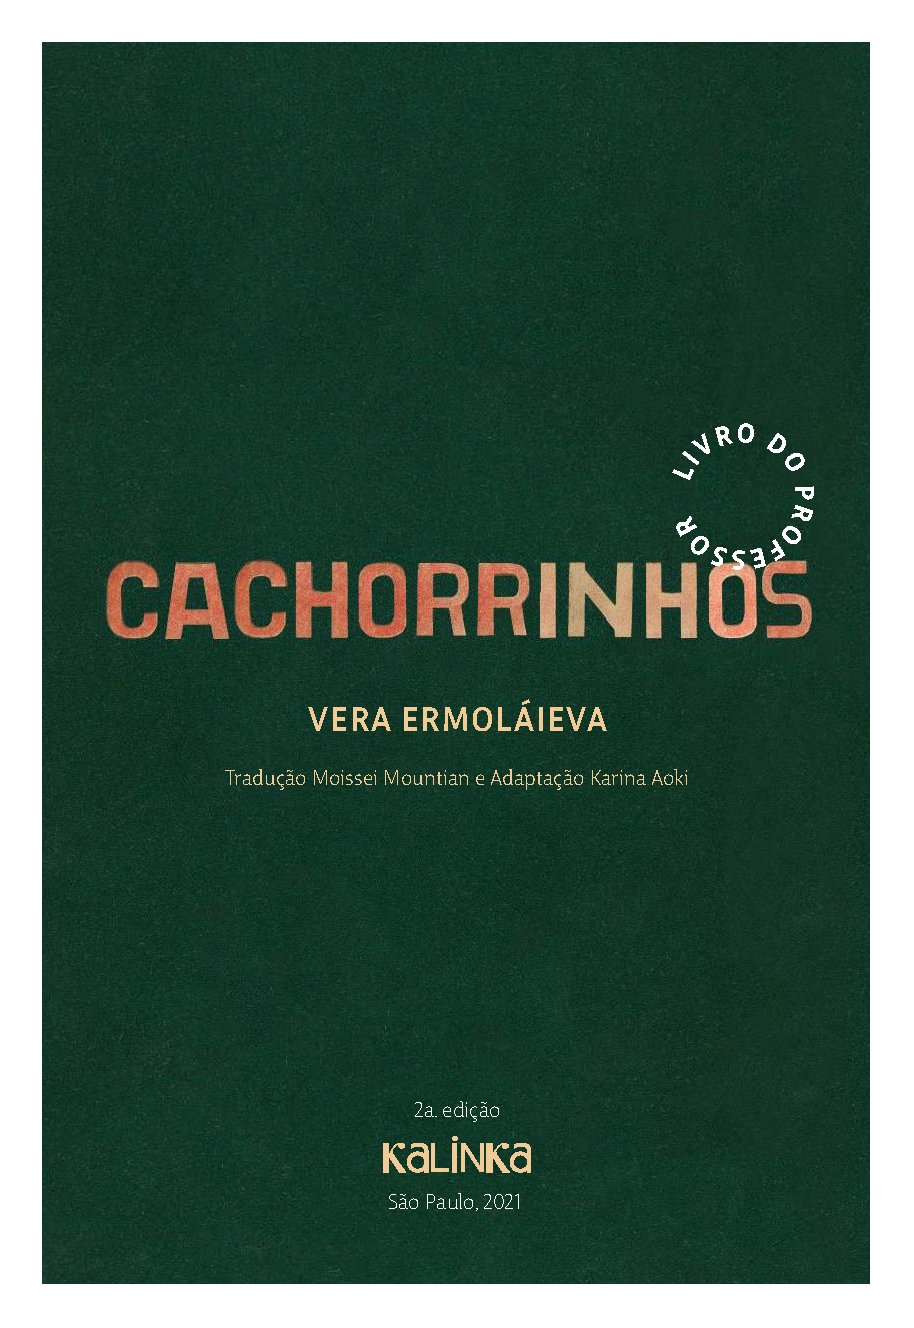
\includepdf[nup=2x2, 					% grid
			% offset=-15mm -5mm, 		% posição
			% scale=.8, 				% tamanho da página
            % delta=4mm 4mm, 			
            % frame,
            % pages={1-4}]{pdfs/PNLD2022-015_MIOLO.pdf}

\end{document}
